\chapter{红外光谱}\label{ch:g11:infrared}

实验室的架子上放着一瓶无色液体，标签
已被撕掉。它可能是醇、酮或酸，三类
化合物装在瓶中时外观完全一样。取一滴样品滴在\omterm{def:g11:infrared:spectrum}{红外光谱}仪的
晶体上，等待两分钟，屏幕上便出现一张
图谱，给出答案。\omterm{def:g7:atoms-and-molecules:molecule}{分子}中的化学键会振动，每一类键吸收
自身频率的红外光，
因此\omterm{def:g11:infrared:spectrum}{红外光谱}就是\omterm{def:g7:atoms-and-molecules:molecule}{分子}中所含化学键的一份清单。

\begin{recall}
\omterm{def:g11:functional-groups:functional-group}{官能团}与\omterm{def:g11:organic-skeletons:organic}{有机化合物}类别（\cref{ch:g11:functional-groups}）。\omterm{def:g11:absorbance:spectrum}{吸收
光谱}表示物质在每个波长处吸收多少光，
（\cref{ch:g11:absorbance}）。\omterm{def:g11:polarity-and-cohesion:hydrogen-bond}{氢键}将 \ce{O-H}
基团与相邻\omterm{def:g7:atoms-and-molecules:molecule}{分子}相连（\cref{ch:g11:polarity-and-cohesion}）。
\end{recall}

\section{化学键的振动}

\omterm{def:g10:lewis-and-shape:covalent-bond}{共价键}并非刚性：两个\omterm{def:g7:atoms-and-molecules:atom}{原子}振动，时而靠近、时而远离，
每秒数万亿次，好比两个小球
用弹簧相连。较硬的弹簧（\omterm{def:g10:lewis-and-shape:multiple-bond}{双键}而非单键）
或较轻的小球（氢\omterm{def:g7:atoms-and-molecules:atom}{原子}而非碳\omterm{def:g7:atoms-and-molecules:atom}{原子}）振动
得更快。化学键能吸收与自身振动频率一致的
红外光，这种红外光肉眼不可见，波长为几微米
至几十微米。

\begin{omfigure}
\begin{tikzpicture}[font=\small]
  \node[aC] (c) at (0,0) {};
  \node[aO] (o) at (2.2,0) {};
  \draw[decorate, decoration={coil, aspect=0.4, segment length=4pt,
    amplitude=4pt}, thick, black!60] (c.east) -- (o.west);
  \draw[<->, omProp, thick] (-0.9,0) -- (-0.45,0);
  \draw[<->, omProp, thick] (2.65,0) -- (3.1,0);
  \node[anchor=north] at (1.1,-0.5) {一根伸缩的键};
  \node[aO] (o1) at (5.3,0) {};
  \node[aH] (h1) at (6.7,0) {};
  \draw[decorate, decoration={coil, aspect=0.4, segment length=3pt,
    amplitude=3pt}, thick, black!60] (o1.east) -- (h1.west);
  \draw[<->, omProp, thick] (7.0,0) -- (7.7,0);
  \node[anchor=north, align=center] at (6.2,-0.5) {较轻的氢原子：\\ 振动更快};
\end{tikzpicture}

{\small 以弹簧连接两个小球表示的键，其振动
频率由键的劲度和\omterm{def:g7:atoms-and-molecules:atom}{原子}的质量决定；
与该频率相同的红外光被吸收。}
\end{omfigure}

\begin{definition}[波数]\label{def:g11:infrared:wavenumber}
光的\emph{波数}\index{波数} $\sigma$ 是其
波长的倒数，$\sigma = 1/\lambda$。在\omterm{def:g11:infrared:spectrum}{红外光谱}中，
它以 \si{cm^{-1}} 为单位，表示
每厘米内所含的波长个数。波数越大，波长越短，
振动越快。
\end{definition}

\begin{example}[由波数求波长]\label{ex:g11:infrared:convert}
位于 $\sigma = \qty{2000}{cm^{-1}}$ 处的吸收带对应
$\lambda = 1/2000 = \qty{5.0e-4}{cm} = \qty{5.0}{\micro m}$。\omterm{def:g11:infrared:spectrum}{红外
光谱}通常从 \qty{4000}{cm^{-1}}（\qty{2.5}{\micro m}）
到 \qty{500}{cm^{-1}}（\qty{20}{\micro m}）。
\end{example}

\section{读懂红外光谱}

\begin{definition}[红外光谱，透射比]\label{def:g11:infrared:spectrum}
样品在给定\omterm{def:g11:infrared:wavenumber}{波数}处的\emph{透射比}\index{透射比} $T$ 是
透过该样品的红外光所占的百分比，
若无任何吸收，则为 \qty{100}{\percent}。
化合物的\emph{红外光谱}\index{红外光谱}是 $T$ 对\omterm{def:g11:infrared:wavenumber}{波数}的图像，
按惯例，图中的\omterm{def:g11:infrared:wavenumber}{波数}
自左至右递减。
\end{definition}

\begin{definition}[吸收带，指纹区]\label{def:g11:infrared:band}
\emph{吸收带}\index{吸收带}是\omterm{def:g11:infrared:spectrum}{透射比}的
一处凹陷：这些\omterm{def:g11:infrared:wavenumber}{波数}的光被某种键吸收。其
位置说明是哪一种键，宽度与深度
则补全图像。约 \qty{1500}{cm^{-1}} 以下，光谱
中密布着依赖整个\omterm{def:g7:atoms-and-molecules:molecule}{分子}的吸收带，这一\emph{指纹区}\index{指纹区}
能通过与已知光谱对照来鉴定化合物，
但难以逐键读出。
\end{definition}

\begin{inthelab}[记录光谱]
目前多数中学和大学的光谱仪都使用小型金刚石晶体：
将一滴液体，或用夹具压紧的少量固体颗粒，
放在晶体上，红外光束掠过其表面，用以探测
样品。先记录洁净晶体的光谱（即“背景”），
它起着空白对照的作用。两次测样之间，晶体
用纸巾和少量\omterm{def:g6:solutions-and-solubility:solute}{溶剂}擦拭干净。
\end{inthelab}

\section{特征吸收带}

\begin{proposition}[每类键都有其吸收带]\label{prop:g11:infrared:bands}
% ledger: ir:OH-free, ir:OH-bonded, ir:OH-acid, ir:NH, ir:CH, ir:CO-aldehyde, ir:CO-ketone, ir:CO-ester, ir:CO-acid, ir:CC-double, ir:CO-single
每类键都吸收于特定的\omterm{def:g11:infrared:wavenumber}{波数}范围，
不同\omterm{def:g7:atoms-and-molecules:molecule}{分子}之间大致相同：
\begin{center}
\small
\begin{tabular}{lll}
\hline
键 & \omterm{def:g11:infrared:wavenumber}{波数}（\si{cm^{-1}}） & 峰形 \\
\hline
\ce{O-H}，未形成\omterm{def:g11:polarity-and-cohesion:hydrogen-bond}{氢键}（气态、稀溶液） & 约 3600 & 尖锐 \\
\ce{O-H}，形成\omterm{def:g11:polarity-and-cohesion:hydrogen-bond}{氢键}（液态醇） & 3300--3400 & 宽、强 \\
\ce{O-H}，\omterm{def:g11:functional-groups:carboxylic-acid}{羧酸}中 & 2500--3300 & 很宽 \\
\ce{N-H}，胺中 & 3300--3500 & 中等（\ce{-NH2} 有两个峰） \\
\ce{C-H}，链上 & 2850--2960 & 强 \\
\ce{C=O}，酯中 & 约 1735 & 很强、尖锐 \\
\ce{C=O}，醛中 & 约 1730 & 很强、尖锐 \\
\ce{C=O}，酮中 & 约 1715 & 很强、尖锐 \\
\ce{C=O}，\omterm{def:g11:functional-groups:carboxylic-acid}{羧酸}中 & 约 1710 & 很强、较宽 \\
\ce{C=C} & 约 1650 & 中等 \\
\ce{C-O}，醇中 & 约 1050 & 强 \\
\hline
\end{tabular}
\end{center}
\end{proposition}

\begin{proof}
这些范围是在许多化合物上测得的。它们按
化学键分组，因为化学键的振动主要取决于化学键本身
及其两个\omterm{def:g7:atoms-and-molecules:atom}{原子}，而很少取决于\omterm{def:g7:atoms-and-molecules:molecule}{分子}的其余部分。
\end{proof}

\begin{omfigure}
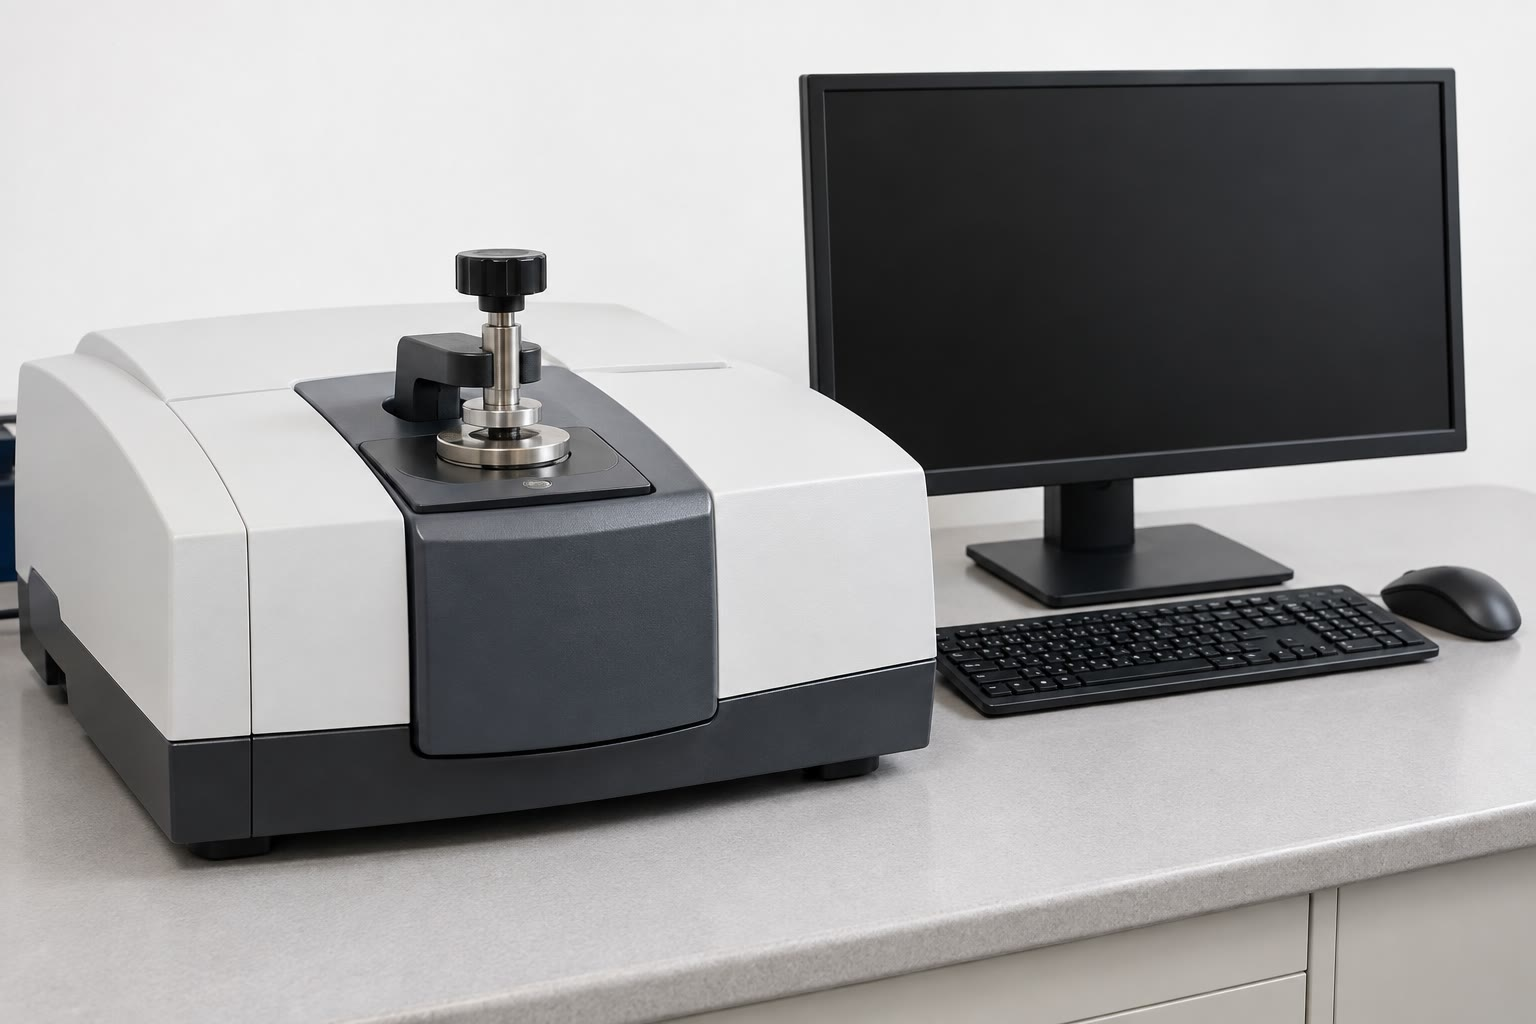
\includegraphics[width=0.48\linewidth]{images/book1/ai/g11-ftir.jpg}

{\small 台式\omterm{def:g11:infrared:spectrum}{红外光谱}仪，连同其晶体和夹具。}
\end{omfigure}

\begin{omfigure}
\begin{tikzpicture}[font=\small, x=0.0036cm, y=0.5cm]
  % wavenumber axis reversed: x = 4000 - sigma
  \fill[black!8] (2500,0.2) rectangle (3500,7.6);
  \node[font=\footnotesize, align=center, black!60] at (3000,6.8) {指纹区};
  \draw[->] (0,0) -- (3600,0) node[right] {$\sigma$};
  \foreach \s in {4000,3500,3000,2500,2000,1500,1000,500}
    \draw ({4000-\s},0) -- ({4000-\s},-0.15) node[below, font=\footnotesize] {\s};
  \node[below=12pt] at (1800,-0.3) {波数（\si{cm^{-1}}）};
  \foreach \a/\b/\y/\c/\l in {
      3600/3600/7/omDef/{\ce{O-H}（游离）},
      3300/3400/6/omDef/{\ce{O-H}（缔合）},
      2500/3300/5/omThm/{\ce{O-H}（羧酸）},
      3300/3500/4/omMeth/{\ce{N-H}},
      2850/2960/3/black!60/{\ce{C-H}},
      1700/1740/2/omProp/{\ce{C=O}},
      1050/1050/1/black!45/{\ce{C-O}}} {
    \fill[\c, rounded corners=1pt] ({4000-\b-12},{\y-0.25}) rectangle ({4000-\a+12},{\y+0.25});
    \node[anchor=west, font=\footnotesize] at ({4000-\a+40},\y) {\l};
  }
\end{tikzpicture}

{\small 主要化学键的吸收位置。\ce{O-H} 和 \ce{N-H} 的吸收带位于
左侧，\ce{C=O} 吸收带通常最强，位于
\qty{1700}{cm^{-1}} 附近；\qty{1500}{cm^{-1}} 以下为
\omterm{def:g11:infrared:band}{指纹区}。}
\end{omfigure}

\begin{proposition}[氢键使 O--H 吸收带变宽]\label{prop:g11:infrared:hbond}
% ledger: ir:OH-free, ir:OH-bonded, ir:ethanol-OH
当 \ce{O-H} 基团以\omterm{def:g11:polarity-and-cohesion:hydrogen-bond}{氢键}相连时，如液态醇中，
吸收带较宽，位于较低\omterm{def:g11:infrared:wavenumber}{波数}处（约
3300--\qty{3400}{cm^{-1}}）；无\omterm{def:g11:polarity-and-cohesion:hydrogen-bond}{氢键}时（如气态），其吸收带尖锐，
位于 \qty{3600}{cm^{-1}} 附近。
\end{proposition}

\begin{proof}
在本阶段不加证明地承认：\omterm{def:g11:polarity-and-cohesion:hydrogen-bond}{氢键}拉动氢\omterm{def:g7:atoms-and-molecules:atom}{原子}，使
\ce{O-H} 键减弱，其振动变慢；由于每个\omterm{def:g7:atoms-and-molecules:molecule}{分子}的成键情况略有不同，
吸收带便展宽成一定范围。
\end{proof}

\section{识别官能团}


\begin{method}[读取红外光谱]\label{met:g11:infrared:reading}
\begin{enumerate}
  \item 先看 \qty{1500}{cm^{-1}} 以上的区域；将\omterm{def:g11:infrared:band}{指纹区}
        留待与已知光谱比对。
  \item \qty{1700}{cm^{-1}} 附近：若吸收带很强，则为 \ce{C=O} 基团
        （醛、酮、\omterm{def:g11:functional-groups:carboxylic-acid}{羧酸}、酯、\omterm{def:g11:functional-groups:amine}{酰胺}）。
  \item 在 2500 与 \qty{3700}{cm^{-1}} 之间：
        \qty{3350}{cm^{-1}} 附近的宽吸收带表示醇中的 \ce{O-H}；
        2500 至 \qty{3300}{cm^{-1}} 的极宽吸收带，若同时含 \ce{C=O}，则为
        \omterm{def:g11:functional-groups:carboxylic-acid}{羧酸}；3300--\qty{3500}{cm^{-1}} 处的中等强度吸收带表示
        \ce{N-H}。
  \item 结合\omterm{def:g11:organic-skeletons:formulas}{分子式}确定化合物类别，
        若有 \ce{C=O} 吸收带，再依其位置核对。
\end{enumerate}
\end{method}

\begin{omfigure}
\newcommand{\irpanel}[2]{%
\begin{tikzpicture}
\begin{axis}[width=0.96\linewidth, height=3.9cm, x dir=reverse, xmin=500,
    xmax=4000, ymin=0, ymax=105, xtick={4000,3000,2000,1000},
    /pgf/number format/1000 sep={},
    ytick={0,50,100}, tick label style={font=\scriptsize},
    label style={font=\scriptsize}, ylabel={$T$ (\%)}, axis lines*=left,
    title={\small #2}, title style={yshift=-4pt}]
  \addplot[thick, omDef] table[x=sigma, y=#1] {figdata/out/grade-11-infrared.dat};
\end{axis}
\end{tikzpicture}}
\begin{minipage}{0.49\linewidth}\irpanel{ethanolL}{A：乙醇（液态）}\end{minipage}\hfill
\begin{minipage}{0.49\linewidth}\irpanel{ethanolG}{B：乙醇（气态）}\end{minipage}

\begin{minipage}{0.49\linewidth}\irpanel{propanone}{C：丙酮}\end{minipage}\hfill
\begin{minipage}{0.49\linewidth}\irpanel{acid}{D：乙酸}\end{minipage}

\begin{minipage}{0.49\linewidth}\irpanel{ester}{E：乙酸乙酯}\end{minipage}\hfill
\begin{minipage}{0.49\linewidth}\irpanel{amine}{F：乙胺}\end{minipage}

{\small 六种化合物的\omterm{def:g11:infrared:spectrum}{红外光谱}，\omterm{def:g11:infrared:wavenumber}{波数}单位为 \si{cm^{-1}}
（\omterm{def:g11:infrared:wavenumber}{波数}向右递减）。本图仅画出本章讨论的吸收带，
其位置取自实测光谱和数据表，
形状由简单模型给出。}
\end{omfigure}

\begin{example}[读取六种光谱]\label{ex:g11:infrared:six}
% ledger: ir:OH-bonded, ir:ethanol-OH, ir:CO-ketone, ir:OH-acid, ir:CO-acid, ir:CO-ester, ir:ethylethanoate-COC, ir:NH
乙醇（A）在 \qty{3350}{cm^{-1}} 附近有一个宽的 \ce{O-H} 吸收带，
\ce{C-H} 吸收带略低于 \qty{3000}{cm^{-1}}，另有一个强的 \ce{C-O}
吸收带位于 \qty{1050}{cm^{-1}} 附近，而 \qty{1700}{cm^{-1}} 附近无吸收。在
气态（B）中，其 \ce{O-H} 吸收带变为一条尖锐谱线，位于
\qty{3666}{cm^{-1}}。丙酮（C）无 \ce{O-H} 吸收带，但有一个很强的
\ce{C=O} 吸收带，位于 \qty{1715}{cm^{-1}}。乙酸（D）两者兼有：一个
极强的 \ce{O-H} 吸收带，位于 2500 至 \qty{3300}{cm^{-1}}，以及一个 \ce{C=O}
吸收带，位于 \qty{1710}{cm^{-1}}。乙酸乙酯（E）的 \ce{C=O} 吸收带位于
\qty{1735}{cm^{-1}}，另有一个强的 \ce{C-O} 吸收带位于 \qty{1240}{cm^{-1}} 附近，且
无 \ce{O-H}。乙胺（F）在
\qty{3300}{cm^{-1}} 以上有两条中等强度的 \ce{N-H} 吸收带。
\end{example}

\section{练习}

\begin{exercise}[$\star$]\label{exo:g11:infrared:1}
将下列\omterm{def:g11:infrared:wavenumber}{波数}换算为以微米为单位的波长：$\sigma = \qty{3300}{cm^{-1}}$
和 $\sigma = \qty{1050}{cm^{-1}}$，哪一个对应较快的
振动？
\end{exercise}

\begin{exercise}[$\star$]\label{exo:g11:infrared:2}
某波长为 \qty{10}{\micro m} 的光被吸收。求其\omterm{def:g11:infrared:wavenumber}{波数}，
以 \si{cm^{-1}} 为单位表示。
\end{exercise}

\begin{exercise}[$\star$]\label{exo:g11:infrared:3}
哪种键会吸收：在 \qty{1715}{cm^{-1}} 附近；在 \qty{3350}{cm^{-1}}
附近（宽峰）；在 2850 至 \qty{2960}{cm^{-1}} 之间？
\end{exercise}

\begin{exercise}[$\star$]\label{exo:g11:infrared:4}
在光谱 C（丙酮）中，找出最强的吸收带。
它属于哪种键？
\end{exercise}

\begin{exercise}[$\star$]\label{exo:g11:infrared:5}
为何\omterm{def:g11:infrared:spectrum}{红外光谱}的纵轴采用\omterm{def:g11:infrared:spectrum}{透射比}，吸收带
朝下？$T = \qty{100}{\percent}$ 表示什么？
\end{exercise}

\begin{exercise}[$\star\star$]\label{exo:g11:infrared:6}
化合物 \ce{C4H8O} 在
\qty{1715}{cm^{-1}} 处有极强吸收带，且在 \qty{3000}{cm^{-1}} 以上无吸收带。另一
化合物 \ce{C4H10O} 在 \qty{3350}{cm^{-1}} 附近有宽吸收带，
\qty{1700}{cm^{-1}} 附近无吸收带。它们分别属于哪类
化合物？为每一种提出一个名称。
\end{exercise}

\begin{exercise}[$\star\star$]\label{exo:g11:infrared:7}
解释为何乙酸的 \ce{O-H} 吸收带如此宽，
甚至比液态乙醇的还宽。
\end{exercise}

\begin{exercise}[$\star\star$]\label{exo:g11:infrared:8}
比较乙醇的光谱 A 和 B。有何变化？原因是什么？
\end{exercise}

\begin{exercise}[$\star\star$]\label{exo:g11:infrared:9}
丙醛和丙酮都是 \ce{C3H6O}，两者都有强的 \ce{C=O}
吸收带。仅凭这一吸收带，\omterm{def:g11:infrared:spectrum}{红外光谱}能否区分它们？还有什么
能提供帮助？
\end{exercise}

\begin{exercise}[$\star\star$]\label{exo:g11:infrared:10}
某化合物在 \qty{1735}{cm^{-1}} 处有一个强吸收带，在
\qty{1240}{cm^{-1}} 附近有一个强吸收带，且 \qty{3000}{cm^{-1}} 以上无吸收带。其\omterm{def:g11:organic-skeletons:formulas}{分子式}为
\ce{C4H8O2}。它属于哪类化合物？乙酸是否可能？丁
酸呢？
\end{exercise}

\begin{exercise}[$\star\star$]\label{exo:g11:infrared:11}
六张光谱中，丙-1-醇\omterm{def:g7:atoms-and-molecules:molecule}{分子}的光谱最像哪一张？
丙酸的呢？请说明理由。
\end{exercise}

\begin{exercise}[$\star\star\star$]\label{exo:g11:infrared:12}
丙-2-醇可被氧化为丙酮。一名学生追踪该
反应，每隔十分钟取样并记录光谱。
描述光谱如何变化。她如何得知反应
已经完成？
\end{exercise}

\begin{exercise}[$\star\star\star$]\label{exo:g11:infrared:13}
丁酸与乙酸乙酯互为\omterm{def:g11:organic-skeletons:isomer}{同分异构体}，均为 \ce{C4H8O2}。描述
它们\omterm{def:g11:infrared:spectrum}{红外光谱}之间的两处差异，并加以解释。
\end{exercise}

\begin{exercise}[$\star\star\star$]\label{exo:g11:infrared:14}
一份乙酸乙酯样品除预期的吸收带外，还显示一个弱的
宽吸收带，位于 \qty{3350}{cm^{-1}} 附近。试提出两种可能导致该吸收带的杂质
（想一想酯如何制得，以及\omterm{def:g4:air-a-mixture-of-gases:air}{空气}中的成分）。
该样品应如何检验？
\end{exercise}

\begin{exercise}[$\star\star\star$]\label{exo:g11:infrared:15}
酮的 \ce{C=O} 吸收带位于 \qty{1715}{cm^{-1}} 附近，
\ce{C=C} 的吸收带位于 \qty{1650}{cm^{-1}} 附近，\ce{C-O} 的吸收带
位于 \qty{1050}{cm^{-1}} 附近。借助两个小球与弹簧的模型，解释
为何\omterm{def:g10:lewis-and-shape:multiple-bond}{双键} \ce{C=O} 的振动比单键 \ce{C-O} 快。为何 \ce{O-H}、\ce{N-H} 与
\ce{C-H} 的吸收带都位于较高的\omterm{def:g11:infrared:wavenumber}{波数}处？
\end{exercise}

\section{周末问题：三个无标签的瓶子}

\begin{problem}[{周末问题——三个瓶子的标签已丢失：
哪个是哪个，以及酮吸收最强的波长是多少？}]
\label{pb:g11:infrared:1}
% ledger: ir:OH-bonded, ir:OH-acid, ir:CO-ketone, ir:CO-acid, ir:CO-single
三个装有无色液体的瓶子标签已丢失。库存清单
上写着瓶中分别为乙醇、丙酮和乙酸。现已记录它们的光谱：
1 号瓶的光谱与 A 相似，2 号瓶与 D 相似，
3 号瓶与 C 相似。

\medskip
\noindent\textbf{第一部分——候选物质。}
\begin{enumerate}
  \item 写出乙醇、丙酮与
        乙酸的\omterm{def:g11:organic-skeletons:formulas}{结构简式}。
  \item 写出它们的\omterm{def:g11:organic-skeletons:formulas}{分子式}。
  \item 写出每种物质所含的\omterm{def:g11:functional-groups:functional-group}{官能团}名称。
  \item 每种物质中哪些键应在
        \qty{1500}{cm^{-1}} 以上产生吸收带？
\end{enumerate}

\medskip
\noindent\textbf{第三部分——光谱。}
\begin{enumerate}[resume]
  \item 1 号瓶：是否存在 \ce{C=O} 吸收带？是否存在 \ce{O-H} 吸收带？
        它是哪种化合物？
  \item 2 号瓶：描述其两个最强的特征。它是哪种化合物？
  \item 3 号瓶：它是哪种化合物？由哪个吸收带决定？
  \item 能否仅凭气味区分它们？
        为何最好不要去闻？
  \item 为何 2 号瓶的 \ce{O-H} 吸收带比 1 号瓶的更宽？
\end{enumerate}

\medskip
\noindent\textbf{第三部分——\omterm{def:g11:organic-skeletons:isomer}{同分异构体}。}
\begin{enumerate}[resume]
  \item 甲醚是乙醇的\omterm{def:g11:organic-skeletons:isomer}{同分异构体}。写出它的\omterm{def:g11:organic-skeletons:formulas}{分子式}，
        其光谱中会缺少乙醇的哪一个吸收带？
  \item 丙醛是丙酮的\omterm{def:g11:organic-skeletons:isomer}{同分异构体}，它们共有哪一个吸收带？
        各自的位置在哪里？
  \item 甲酸甲酯（\ce{HCOO-CH3}）是乙酸的\omterm{def:g11:organic-skeletons:isomer}{同分异构体}。
        乙酸的哪一个吸收带会缺失？其
        \ce{C=O} 吸收带应位于何处？
  \item 为何仅凭\omterm{def:g11:organic-skeletons:formulas}{分子式}不能确定化合物，而
        结合\omterm{def:g11:organic-skeletons:formulas}{分子式}与光谱通常就能确定？
\end{enumerate}

\medskip
\noindent\textbf{第四部分——波长。}
\begin{enumerate}[resume]
  \item 丙酮最强吸收带的\omterm{def:g11:infrared:wavenumber}{波数}是多少？
  \item 用 \si{m^{-1}} 表示它。
  \item 计算所吸收光的波长，先以米为单位，
        再以微米为单位。
  \item 该光是否可见？它属于
        哪一类辐射？
  \item 对乙醇中位于
        \qty{1050}{cm^{-1}} 附近的 \ce{C-O} 吸收带做同样计算。
  \item 两种键中哪一种振动得更快？
  \item 给出最终结果：丙酮中 \ce{C=O} 键
        吸收最强的波长为多少？
\end{enumerate}
\end{problem}
